\documentclass[11pt,a4paper]{article}
\usepackage[margin=25mm]{geometry}
\usepackage{amsmath,amssymb,amsthm,mathtools,booktabs,graphicx}
\usepackage[T1]{fontenc}
\usepackage{lmodern,microtype}
\usepackage[hidelinks]{hyperref}
\usepackage{enumitem}
\numberwithin{equation}{section}
\renewcommand{\thesection}{\Roman{section}}
\renewcommand{\thesubsection}{\Alph{subsection}}
\newtheorem{assumption}{Assumption}
\newtheorem{proposition}{Proposition}
\newtheorem{theorem}{Theorem}
\newtheorem{lemma}{Lemma}
\theoremstyle{remark}\newtheorem{remark}{Remark}
\newcommand{\R}{\mathbb R}
\newcommand{\norm}[1]{\left\lVert#1\right\rVert}
\newcommand{\diag}{\operatorname{diag}}
\newcommand{\sym}{\operatorname{sym}}
\newcommand{\cW}{\mathcal W}
\newcommand{\cD}{\mathcal D}
\title{State-Dependent Uncertainty Bounds for Robust Output-Feedback MPC\\\large Derivation and a Falcon Certificate-Reuse Numerical Example}
\author{Research draft}
\date{23 September 2026}
\begin{document}
\maketitle
\begin{abstract}
We study state-dependent process uncertainty in a continuous-time output-feedback tube MPC formulation. Starting from a fixed quadratic observer certificate, a Schur-complement construction reduces its auxiliary process envelope for nested local disturbance sets without changing the metric or gains. This yields coupled prediction equations for a squared estimation-error bound and an observer-to-nominal tracking radius. We state conditional recursive-feasibility and robust-constraint-satisfaction guarantees for a free-center MPC formulation, following the architecture of K\"ohler, M\"uller, and Allg\"ower. A Falcon numerical example reuses existing offline certificates and gives a 6.68\% final-time estimation-radius reduction relative to the baseline-equivalent global propagation. The experiment concerns radius dynamics under a prescribed speed schedule; it is not a closed-loop plant simulation. Continuous-domain certification, rigorous numerical residual treatment, local uncertainty validation, and a nonempty compatible terminal set remain unresolved.
\end{abstract}

\section{Introduction}
Robust output-feedback MPC must account for both uncertain state estimates and deviations between an observer trajectory and a nominal prediction. A global uncertainty envelope can be unnecessarily conservative in operating regions with smaller model mismatch. Our objective is to retain an existing offline design while allowing the predicted uncertainty allowance to depend on the operating region covered by the error tubes.

The organization follows \cite{kohler2021}: preliminaries, estimation bounds, robust output-feedback MPC, and a numerical example. Joint nominal and tube prediction, a free nominal initial center, and shifted-candidate arguments are established ingredients of Section IV-B of that reference. They are not claimed as new here. Our proposed extension concerns the local process-envelope construction and its incorporation into coupled continuous-time radius dynamics. No novelty claim relative to the broader literature is established by this draft.

\subsection{Scope and status}
The analysis uses fixed metrics and observer/controller gains, a fixed regulation target, and time-invariant constraints. Measurement noise remains globally bounded in the numerical example. The state-dependent process model is prescribed synthetically; containment inside a global uncertainty set does not establish that the actual plant disturbance belongs to the smaller local set. The theorems below are conditional mathematical statements, while the Falcon results are finite numerical audits of saved certificates. The full planning/tracking ROHMPC hierarchy is outside this scope.

\section{Preliminaries}
\subsection{Plant, observer, and nominal prediction}
Consider
\begin{subequations}\label{eq:system}
\begin{align}
\dot x &= f_0(x,u)+E_0D(a(x))w, & w&\in\cW_0,\\
y &= Cx+F\eta, &\eta&\in\mathcal N,\\
\dot{\hat x}&=f_0(\hat x,u)+L(y-C\hat x),\\
\dot z&=f_0(z,v), & u&=v+K(\hat x-z).
\end{align}
\end{subequations}
Here $v$ is the nominal control input, not velocity. The function $f_0$ includes the identified constant bias; only centered residual uncertainty is scaled. The set $\cW_0$ is a centered box and $D(a)$ is diagonal, scaling selected channels by $a\in[\beta,1]$ and leaving the others unchanged, with $0<\beta<1$. Thus $E_0D(a)\cW_0$ is nested as $a$ increases. The matrix $L$ is a fixed Luenberger observer gain.

Let $P=P_\delta\succ0$, $X=P^{-1}$, and $T^\top T=P$. Define
\begin{equation}
e=x-\hat x,\quad \delta=\hat x-z,\quad V_e=e^\top Pe,\quad
V_e\le R,\quad \norm{\delta}_P\le s.
\end{equation}
$R$ is a squared radius and $r=\sqrt R$ is a radius; neither denotes the true estimation error. The symbol $P$ is distinct from a terminal-cost matrix. Since $x-z=e+\delta$,
\begin{equation}\label{eq:total}
\norm{x-z}_P\le\sqrt R+s.
\end{equation}
Subtracting the dynamics gives
\begin{subequations}\label{eq:errors}
\begin{align}
\dot e&=f_0(x,u)-f_0(\hat x,u)-LCe+E_0D(a)w-LF\eta,\\
\dot\delta&=f_0(\hat x,u)-f_0(z,v)+LCe+LF\eta.
\end{align}
\end{subequations}
Process disturbance enters the estimation error directly. It influences observer-to-nominal tracking indirectly through $e$; the observer equation itself contains no additive plant process disturbance.

\subsection{Domain and incremental conditions}
\begin{assumption}[Regularity and certificate domain]\label{ass:domain}
The model and observer admit unique solutions for admissible measurable disturbances and controls. The derivative inequalities used below hold throughout a neighborhood of the certified state/input domain $\cD$, including every segment needed for incremental arguments. The MPC enforces containment of the true-state tube, observer-state tube, and relevant feedback inputs in this domain at every prediction time.
\end{assumption}
For differentiable $f_0$, its difference at two states with the same input equals a segment-averaged Jacobian times their difference. Consequently, Jacobian LMIs at isolated grid points do not by themselves establish Assumption~\ref{ass:domain}.

\section{State-Dependent Estimation Error Bounds}
\subsection{Recovering the global quadratic certificate}
For $b\in\R^n$, introduce the symmetric off-diagonal block
\begin{equation}
\mathcal S(b)=\begin{bmatrix}0&b\\b^\top&0\end{bmatrix}.
\end{equation}
Let $A_o=A-LC$ and $q_0=\lambda\epsilon^2$, with $\lambda>0$. The saved observer certificate has auxiliary matrices $W,H$ satisfying
\begin{subequations}\label{eq:lmis}
\begin{align}
\mathcal S(E_0w)&\preceq W &&\forall w\in\cW_0,\\
\mathcal S(-LF\eta)&\preceq H &&\forall\eta\in\mathcal N,\\
W+H+\begin{bmatrix}XA_o^\top+A_oX+\lambda X&0\\0&-q_0\end{bmatrix}&\preceq0.
\end{align}
\end{subequations}
The last inequality must hold for all relevant Jacobians. Since $X$ is constant, its time derivative is zero. In the implementation $W$ and $H$ are \texttt{W\_bar} and \texttt{H1\_bar}, respectively.

To see explicitly how these LMIs imply the error bound, first consider the global process envelope ($a=1$). Equation~\eqref{eq:errors} can be written as
\[
\dot e=A_oe+b,\qquad b:=E_0w-LF\eta.
\]
For the nonlinear model, $A$ here is the segment-averaged state Jacobian between $\hat x$ and $x$ at the common input $u$. The following argument applies if the Jacobian LMI holds along that segment. The vector $b$ is the combined process and measurement-noise contribution; it is symbolic, not a measured or numerically substituted disturbance.

Rewrite the first two inequalities in \eqref{eq:lmis} as $\mathcal S(E_0w)-W\preceq0$ and $\mathcal S(-LF\eta)-H\preceq0$, and add the third. The auxiliary matrices cancel:
\[
\underbrace{\mathcal S(E_0w)-W}_{\preceq0}
+\underbrace{\mathcal S(-LF\eta)-H}_{\preceq0}
+\underbrace{W+H+\diag(XA_o^\top+A_oX+\lambda X,-q_0)}_{\preceq0}
\preceq0.
\]
Since $\mathcal S$ is linear,
\[
\mathcal S(E_0w)+\mathcal S(-LF\eta)=\mathcal S(b),
\]
so the resulting matrix inequality is
\[
M:=\begin{bmatrix}
XA_o^\top+A_oX+\lambda X&b\\
b^\top&-q_0
\end{bmatrix}\preceq0.
\]
Negative semidefiniteness means $\xi^\top M\xi\le0$ for every vector $\xi$. Choose $\xi=[Pe;1]$; this does not replace $X$, which remains $P^{-1}$. Using $PX=XP=I$ and constant $P$ gives
\begin{align*}
\begin{bmatrix}Pe\\1\end{bmatrix}^{\!\top}M\begin{bmatrix}Pe\\1\end{bmatrix}
&=e^\top P(XA_o^\top+A_oX+\lambda X)Pe+2e^\top Pb-q_0\\
&=e^\top(A_o^\top P+PA_o)e+2e^\top Pb+\lambda e^\top Pe-q_0\\
&=\dot V_e+\lambda V_e-q_0\le0.
\end{align*}
Therefore,
\begin{equation}\label{eq:global-dissipation}
\dot V_e\le-\lambda V_e+q_0.
\end{equation}
Equivalently, define the invertible matrix $G=\diag(P,1)$. The congruence transformation of $M$ by $G$ is
\begin{equation}\label{eq:observer-congruence}
G^\top MG=
\begin{bmatrix}A_o^\top P+PA_o+\lambda P&Pb\\b^\top P&-q_0\end{bmatrix}\preceq0.
\end{equation}
Indeed, $v^\top G^\top MGv=(Gv)^\top M(Gv)\le0$ for every $v$; invertibility makes the two matrix inequalities equivalent. Evaluating the transformed matrix at $[e;1]$ is identical to evaluating $M$ at $[Pe;1]$, because $G[e;1]=[Pe;1]$. The bottom entry $1$ generates the cross term $2e^\top Pb$ and the constant $-q_0$. All these statements hold for every admissible $w,\eta$ without knowing their actual values online.

The comparison equation $\dot R=-\lambda R+q_0$ has solution
\begin{equation}\label{eq:global-solution}
R(t)=\epsilon^2+(R(0)-\epsilon^2)e^{-\lambda t}.
\end{equation}
When $R(0)\ge V_e(0)$ it bounds the estimation error; when $R(0)=\epsilon^2$, it exactly recovers the original constant radius $\epsilon$.

\subsection{Local process-envelope reduction}
Partition the saved matrix as
\begin{equation}
W=\begin{bmatrix}Q&h_w\\h_w^\top&c\end{bmatrix},\qquad Q\succ0.
\end{equation}
The Schur complement gives
\begin{equation}\label{eq:schur}
\mathcal S(E_0D(a)w)\preceq W
\iff (E_0D(a)w-h_w)^\top Q^{-1}(E_0D(a)w-h_w)\le c.
\end{equation}
Define
\begin{equation}
g(a)=\max_{w\in\operatorname{vert}(\cW_0)}
(E_0D(a)w-h_w)^\top Q^{-1}(E_0D(a)w-h_w).
\end{equation}
The vertex maximum covers the entire box because the quadratic is convex in $w$. Each vertex expression is convex in $a$, since $D(a)$ is affine. Their maximum $g$ is therefore convex. Nestedness additionally implies $g(\beta)\le g(1)$. For $a\in[\beta,1]$,
\begin{equation}\label{eq:chord}
g(a)\le g(1)-\frac{1-a}{1-\beta}\bigl(g(1)-g(\beta)\bigr).
\end{equation}
\begin{proposition}[Local forcing from a fixed certificate]\label{prop:local}
Assume \eqref{eq:lmis} holds exactly and $Q\succ0$. Choose
$0\le\Delta\le g(1)-g(\beta)$ and define
\begin{align}
\theta(a)&=\frac{1-a}{1-\beta},\\
W(a)&=\begin{bmatrix}Q&h_w\\h_w^\top&c-\Delta\theta(a)\end{bmatrix},\\
q(a)&=q_0-\Delta\theta(a).\label{eq:q}
\end{align}
Then $W(a)$ covers the local process set and the derivative bound becomes
$\dot V_e\le-\lambda V_e+q(a)$.
\end{proposition}
\begin{proof}
The global certificate implies $c\ge g(1)$. Equation~\eqref{eq:chord} and the choice of $\Delta$ give $g(a)\le c-\Delta\theta(a)$, proving the local envelope inequality by \eqref{eq:schur}. In the final LMI, reducing the bottom-right entry of $W$ by $\Delta\theta(a)$ is exactly cancelled by replacing $-q_0$ with $-q(a)$. Its other entries are unchanged. The quadratic-form argument for \eqref{eq:global-dissipation} then applies.
\end{proof}
At $a=1$ the global certificate is recovered. This construction changes an auxiliary envelope, not $P,K,L$, and requires no new SDP. For the subsequent formulation we additionally require $q_0-\Delta>0$.

\subsection{Bounding the unknown operating point}
For the velocity-dependent example, let $S_v$ select translational velocity and set
\begin{equation}
a(x)=\beta+(1-\beta)\frac{\norm{S_vx}_2^2}{v_{\max}^2},\qquad
\norm{S_vx}_2\le v_{\max}.
\end{equation}
Since $\norm{S_ve}_2\le\norm{S_vT^{-1}}_2\norm e_P$, define
\begin{align}
c_v&=\norm{S_vT^{-1}}_2,\\
v_{\rm up}&=\min\{v_{\max},\norm{S_vz}_2+c_v(\sqrt R+s)\},\\
a_{\rm up}&=\beta+(1-\beta)(v_{\rm up}/v_{\max})^2.
\end{align}
The cap is valid only if the true-state velocity domain is guaranteed. Nominal feasibility alone does not justify it. Nestedness allows use of the process envelope at $a_{\rm up}$ for every true state in the tube. Write $q(z,R,s)=q(a_{\rm up})$.

\subsection{Earlier separate-norm prototype}
An initial alternative bounded process and noise channels separately:
\begin{equation}
\dot r=-\rho_o r+b_{\rm rest}+a_{\rm up}b_{\rm acc}+b_\eta.
\end{equation}
For example $b_{\rm acc}=\max\norm{TE_{\rm acc}w_{\rm acc}}_2$ and
$b_\eta=\max_{\eta\in\mathcal N}\norm{TLF\eta}_2$.
The triangle inequality bounds the norm of a sum by the sum of separate maxima. This can discard joint directional information. The resulting bound need not recover the original SDP radius even when $a=1$. Proposition~\ref{prop:local} was introduced to preserve the original quadratic certificate instead.

\section{Robust Output-Feedback MPC}
\subsection{Coupled tube dynamics}
Suppose the tracking contraction condition holds throughout the relevant segments:
\begin{equation}
(A+BK)^\top P+P(A+BK)\preceq-2\rho P,\qquad\rho>0.
\end{equation}
With $\gamma=\norm{TLC T^{-1}}_2$ and $b_\eta$ as above, \eqref{eq:errors} implies
\begin{equation}
D^+\norm\delta_P\le-\rho\norm\delta_P+\gamma\sqrt{V_e}+b_\eta.
\end{equation}
Thus the proposed augmented prediction is
\begin{subequations}\label{eq:tubes}
\begin{align}
\dot z&=f_0(z,v),\\
\dot R&=-\lambda R+q(z,v,R,s),\\
\dot s&=-\rho s+\gamma\sqrt R+b_\eta.
\end{align}
\end{subequations}
The general notation permits input dependence in $q$; the present velocity example has none explicitly. The forcing must bound the entire state/input tube, not only its nominal center.

\begin{assumption}[Radius regularity and initial bounds]\label{ass:radii}
On the admissible augmented domain $q$ is locally Lipschitz and
$0<q_{\min}\le q\le q_{\max}$. Define
\begin{equation}
0<R_{\min}\le q_{\min}/\lambda,\quad R_{\max}=q_{\max}/\lambda,\quad
s_{\max}=(\gamma\sqrt{R_{\max}}+b_\eta)/\rho.
\end{equation}
The radii lie in $\mathcal B=[R_{\min},R_{\max}]\times[0,s_{\max}]$. An available initial prior $\bar R_0$ satisfies $V_e(0)\le\bar R_0$. The observer is continuous across updates; observer resets require a separately certified jump rule.
\end{assumption}
The vector field points inward on every boundary of $\mathcal B$, so this set is invariant along admissible nominal trajectories. The positive lower radius avoids the lack of local Lipschitz continuity of $\sqrt R$ at zero. Cases with $q_{\min}=0$ require separate analysis.

\begin{lemma}[Tube containment]\label{lem:tube}
Under Assumptions~\ref{ass:domain}--\ref{ass:radii}, the observer and tracking derivative inequalities, and valid initial bounds, $V_e(t)\le R(t)$ and $\norm{\delta(t)}_P\le s(t)$ throughout an applied prediction interval.
\end{lemma}
\begin{proof}
On $V_e=R$, the derivative of $V_e-R$ is nonpositive. On $\norm\delta_P=s$ with $V_e\le R$,
$D^+(\norm\delta_P-s)\le\gamma(\sqrt{V_e}-\sqrt R)\le0$.
The regularity assumptions and tangent/comparison argument yield invariance of the coupled tube. Domain inclusion and a first-exit continuation argument ensure that the derivative hypotheses remain applicable.
\end{proof}
For the same nominal signal and initial radii, $q\le q_0$ also implies $R_{\rm local}\le R_{\rm global}$ by a scalar integrating-factor comparison, and then $s_{\rm local}\le s_{\rm global}$. This compares bounds, not actual errors or MPC performance.

\subsection{Tightened constraints and MPC initialization}
For each mixed constraint $g_j(x,u)\le0$, impose
\begin{equation}\label{eq:tightening}
\sup_{\norm e_P\le\sqrt R,\ \norm\delta_P\le s}
 g_j(z+\delta+e,v+K\delta)\le0.
\end{equation}
For $a_j^\top x+b_j^\top u\le c_j$, the exact support-function form is
\begin{equation}
a_j^\top z+b_j^\top v+
orm{(a_j^\top+b_j^\top K)T^{-1}}_2s
+
orm{a_j^\top T^{-1}}_2\sqrt R\le c_j.
\end{equation}
All tube/domain constraints hold continuously over the prediction horizon. An implementation using only shooting or collocation nodes needs an intersample guarantee.

Let $H_p>0$ be the horizon and $0<h\le H_p$ the sampling period. At update $k$, minimize
\begin{equation}\label{eq:cost}
J_k=\int_0^{H_p}\ell(z(\tau),v(\tau))\,d\tau+V_f(z(H_p))
\end{equation}
subject to \eqref{eq:tubes}, \eqref{eq:tightening}, domain inclusion, $(R,s)\in\mathcal B$, and
\begin{equation}\label{eq:init}
R(0)=\bar R_k,\qquad\norm{\hat x_k-z(0)}_P\le s(0),\qquad
(z(H_p),R(H_p),s(H_p))\in\Omega_f.
\end{equation}
The initial nominal center is free. Apply $u=v_k^*(\tau)+K(\hat x-z_k^*(\tau))$ for $0\le\tau<h$, and carry $\bar R_{k+1}=R_k^*(h)$. Superscript $*$ denotes the selected plan; optimality is needed only for the optimal-value assertion below.

\subsection{Terminal ingredients and conditional guarantees}
\begin{assumption}[Terminal ingredients]\label{ass:terminal}
There exist a nonempty nominal terminal set $Z_f$ and controller $\kappa_f$ such that $\dot z=f_0(z,\kappa_f(z))$ leaves $Z_f$ invariant. For every $z\in Z_f$, the tightened and domain constraints hold at $R_{\max},s_{\max}$. For the cost assertion additionally assume $\ell,V_f\ge0$ and
\begin{equation}\label{eq:terminalcost}
\nabla V_f(z)f_0(z,\kappa_f(z))\le-\ell(z,\kappa_f(z)).
\end{equation}
\end{assumption}
Then $\Omega_f=Z_f\times\mathcal B$ is invariant under terminal control and the radius dynamics. This construction uses global radii only to certify the terminal set; local radii are retained along the horizon.

\begin{theorem}[Conditional closed-loop properties]\label{thm:mpc}
Suppose Assumptions~\ref{ass:domain}--\ref{ass:terminal} and the derivative inequalities hold exactly, and the initial MPC problem is feasible. Applying a feasible plan and the update \eqref{eq:init} at each sample gives recursive feasibility and continuous-time robust constraint satisfaction for all disturbances in the assumed sets. If \eqref{eq:terminalcost} holds and attained global minimizers are used, then
\begin{equation}\label{eq:decrease}
J_{k+1}^*\le J_k^*-\int_0^h\ell(z_k^*(\tau),v_k^*(\tau))\,d\tau.
\end{equation}
\end{theorem}
\begin{proof}
Shift the previous nominal input/state and both radius trajectories by $h$ on $[0,H_p-h]$. The carried prior makes the initial $R$ equality hold; Lemma~\ref{lem:tube} gives $\norm{\hat x_{k+1}-z_k^*(h)}_P\le s_k^*(h)$. Time invariance preserves the remaining constraints and dynamics. Append the terminal controller and radius dynamics for the final $h$ units of time. Terminal invariance gives a feasible tail and endpoint. Induction proves recursive feasibility. Lemma~\ref{lem:tube} and \eqref{eq:tightening} give actual constraint satisfaction on each applied interval. Integrating \eqref{eq:terminalcost} over the tail bounds its cost by the previous terminal cost; cancellation of the common horizon portion and optimality give \eqref{eq:decrease}.
\end{proof}
A feasible fallback suffices for feasibility. A suboptimal solver preserves the analogous selected-plan cost decrease if its accepted cost is no larger than the shifted candidate cost. Radius penalties are absent from \eqref{eq:cost}; including them requires a compatible augmented terminal-cost inequality.

\begin{remark}[Relation to Section IV of \cite{kohler2021}]
Equation (26) of that paper predicts nominal states/inputs and both error bounds with a free initial nominal center. Its Theorem 4 uses monotonicity and nestedness when online updates reduce the initial bounds. Our conservative bookkeeping carries the predicted estimation bound exactly and permits the old tracking bound, so an identical shifted radius trajectory is feasible without this extra comparison step. Its Section IV-C treats resetting the nominal center using a different candidate and stronger terminal conditions; the present theorem does not establish that reset variant. Unlike its discrete-time global-forcing prediction, the proposed $q$ depends on the predicted operating tube.
\end{remark}
The value decrease alone is not a full true-state asymptotic-stability theorem: nominal recentering can introduce jumps, and persistent uncertainty remains. Equation~\eqref{eq:total} gives
$\norm{x-x_{\rm ref}}_P\le\norm{z-x_{\rm ref}}_P+\sqrt R+s$.
Further convergence assumptions and analysis are needed for a practical-stability conclusion.

\section{Numerical Example: Falcon Model}
\subsection{Model and reproduced offline design}
The example uses the repository \cite{rohmpc} and the saved Falcon design from 10 September 2026. The 12-state model consists of position, attitude, translational velocity, and body angular velocity, with four rotor inputs. The nominal translational drag matrix is zero in this instance. Its Jacobians are therefore independent of translational velocity; this does not restrict the controller to hovering. The velocity domain is $[-2,2]^3$ m/s, giving $v_{\max}=\sqrt{12}$ m/s.

The original 1024-point Jacobian grid varies four rotor inputs, three angles, and three body rates at two endpoints each. Positions and translational velocities are zero at these points. This grid alone does not certify the continuous domain of the remaining nonlinear coordinates.

The reproduced robust-design and terminal-cost SDPs returned \texttt{OPTIMAL}, with objectives 1494.858118 and 38.564610, respectively. The first is a weighted combination of normalized squared tightening coefficients and squared estimation radius, not an optimized contraction rate. The second minimizes the trace of the terminal-cost matrix. Solver success does not ensure useful tightened constraints: the reproduced motor-input half-width was approximately 0.1200, whereas the associated global margin was 0.4619, leaving negative available width. Consequently, this design has not supplied the nonempty terminal set required by Theorem~\ref{thm:mpc}.

\subsection{Prescribed local uncertainty and parameters}
Only the centered acceleration disturbance channels 7--9 are scaled. Other process channels, measurement noise, and the nominal bias remain unchanged. We use $\beta=0.25$ and the velocity law in Section III-C. This is a synthetic uncertainty model, not a new identification or UQ result. The experiment reuses the saved $X,P,L,K,W,H,\lambda$ and solves no new SDP.
\begin{table}[htbp]\centering
\caption{Saved certificate and local-envelope parameters (rounded).}
\begin{tabular}{lr}\toprule
Quantity & Value\\\midrule
Observer decay coefficient $\lambda$ & 0.497029\\
Original uncalibrated $\epsilon$ & 0.07442638619\\
Global forcing $q_0$ & 0.002753187883\\
$g(1)$ & 0.00148773\\
$g(\beta)$ & 0.00104178\\
$\Delta=0.99[g(1)-g(\beta)]$ & 0.000441487\\
$q(\beta)$ & 0.0023117\\
Condition number of $Q$ & 3474.67\\\bottomrule
\end{tabular}\label{tab:parameters}
\end{table}
The factor 0.99 retains a numerical cushion but does not repair an infeasible baseline certificate or provide a rigorous floating-point error bound.

\subsection{Radius propagation experiment}
A prescribed nominal speed is 0 m/s on $[0,8)$ s, 2.5 m/s on $[8,16)$ s, and 0 m/s on $[16,32]$ s. Initialize $R(0)=\epsilon^2$, $s(0)=0$. Both cases use identical metrics, gains, initial bounds, tracking dynamics, and noise; only the local forcing versus $q_0$ changes. The global estimation radius equals $\epsilon$ by \eqref{eq:global-solution}.
\begin{table}[htbp]\centering
\caption{Final-time comparison at 32 s; these are bounds, not measured errors.}
\begin{tabular}{lrr}\toprule
Quantity & Global & State-dependent\\\midrule
Estimation radius $r$ & 0.07442638619 & 0.06945456129\\
Tracking radius $s$ & 0.392384 & 0.367532\\\bottomrule
\end{tabular}\label{tab:results}
\end{table}
The final estimation-radius reduction is $100(1-r_{\rm local}/\epsilon)=6.68019\%$. This is neither a time-average improvement nor a universal performance guarantee. The speed schedule is not a dynamically feasible quadrotor trajectory, and no MPC optimization or closed-loop plant simulation is performed.
\begin{figure}[htbp]\centering
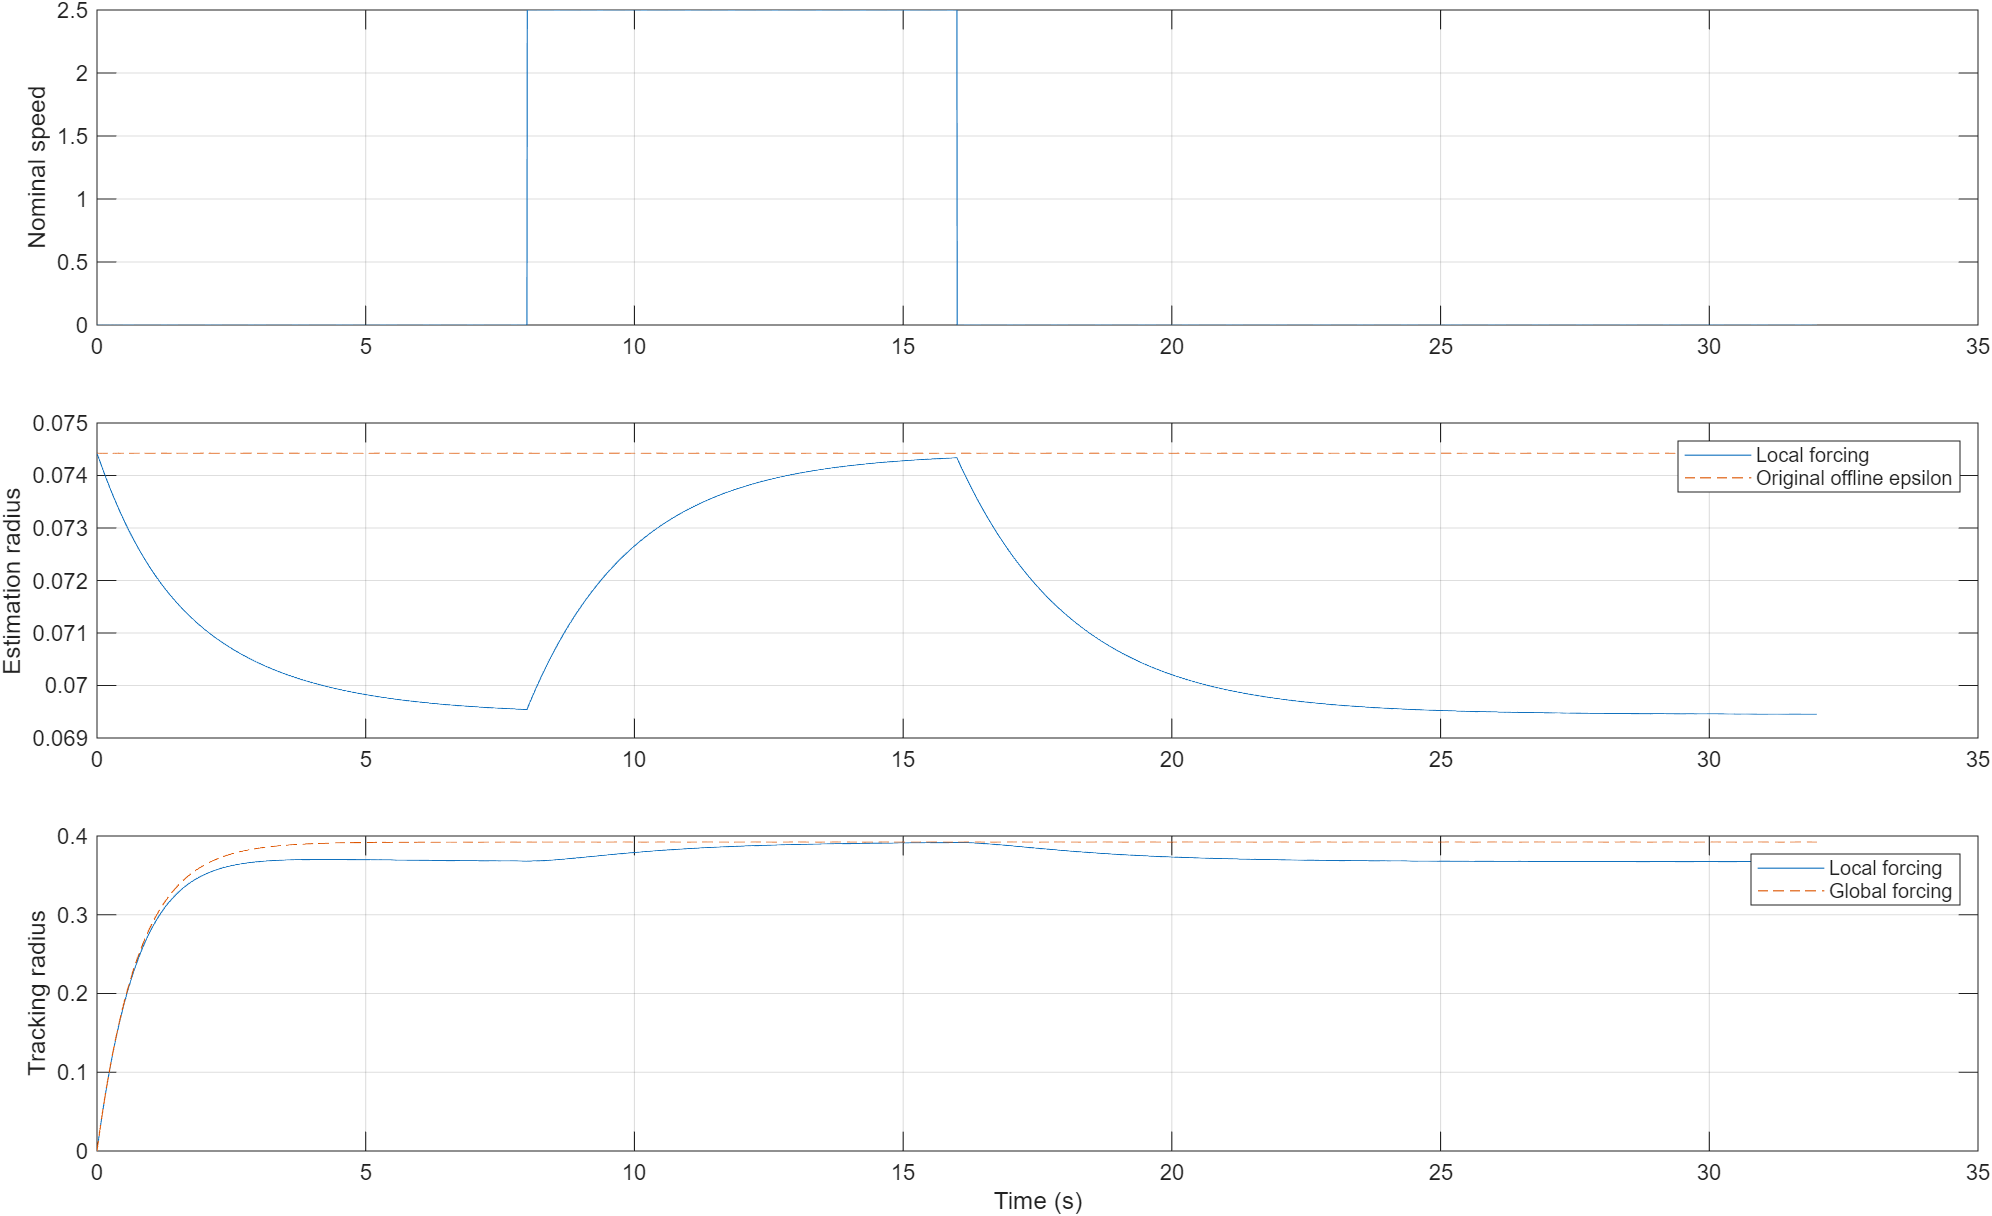
\includegraphics[width=0.96\linewidth]{falcon_tube_comparison.png}
\caption{Recorded tube-ODE experiment with a prescribed low/high/low nominal-speed schedule. The figure is copied from the saved run, not generated by a closed-loop simulator.}\label{fig:tubes}
\end{figure}
The earlier separate-norm prototype produced a global equilibrium radius of approximately 0.105718 and a final local radius of 0.0979251, both above the original 0.0744264. These values belong to a different bound construction and do not indicate empirical calibration of the original $\epsilon$. The quadratic-envelope approach restores a baseline-equivalent comparison.

\subsection{Numerical checks and limitations}
The current experiment checks all 4096 original process vertices, all noise vertices, the 1024 original dynamics points, and all process vertices at 31 scale values. It additionally evaluates 1968 admissible random nonlinear error configurations. Table~\ref{tab:residuals} reports the saved residuals.
\begin{table}[htbp]\centering
\caption{Numerical audit; positive matrix residuals are tolerated numerically, not exact certificates.}
\begin{tabular}{lr}\toprule
Check & Maximum residual\\\midrule
Original process-envelope LMI & $+5.50832\,10^{-8}$\\
Original noise-envelope LMI & $+5.57035\,10^{-8}$\\
Observer dynamics LMI & $+5.45468\,10^{-8}$\\
Tracking LMI & $-0.0030671$\\
Local Schur envelope & $+5.63813\,10^{-8}$\\
Sampled nonlinear derivative excess & $-0.00229595$\\\bottomrule
\end{tabular}\label{tab:residuals}
\end{table}
The saved feasibility tolerance is $10^{-6}$. Small positive residuals mean feasibility within that numerical tolerance, not exact semidefinite feasibility. The convex-chord argument covers intermediate scales analytically only conditional on exact baseline inequalities. Finite Jacobian and nonlinear samples do not prove full-domain coverage. No closed-loop feasibility, safety, or stability claim for Falcon follows from these tests.

\section{Conclusion}
A fixed observer certificate can support locally reduced process forcing through a Schur-complement envelope construction. Coupling this forcing to a tracking radius yields a candidate state-dependent output-feedback MPC formulation with conditional recursive-feasibility and safety guarantees. The Falcon radius experiment demonstrates a smaller local bound relative to a baseline-equivalent global propagation. Remaining work is to certify the continuous domain and numerical margins, validate the local uncertainty model, construct compatible nonempty terminal ingredients, and then implement and evaluate the closed-loop controller.

\appendix
\section{Reproducibility and Source Map}
All paths below are relative to the repository root. The baseline is
\path{work/offline-sanity-20260910/offline_design.mat}.
The current script is \path{research/state_dependent_bounds/run_lmi_radius_recovery.m}.
The reported run is \path{research/state_dependent_bounds/results/lmi_20260910_222354/}, containing \path{run.log}, \path{lmi_radius_result.mat}, \path{lmi_radius_comparison.csv}, and the plotted PNG. The older prototype is \path{run_dynamic_bound_demo.m} in the same research directory. The derivation and conditional theorem were developed in \path{LMI_RADIUS_DERIVATION.md} and \path{CLOSED_LOOP_PROOF_FRAMEWORK.md}.

The upstream offline folder is
\path{src/catkin_ws/src/mpc/mpc_solver/scripts/include/offline_computations/mpc-sdp/}.
Its \path{main.m} orchestrates the design;
\path{compute_Pdelta_Kdelta_cs_co.m} computes the main robust design;
\path{compute_check_epsilon_RPI_LMIs.m} supplies the observer-envelope inequalities;
\path{compute_w_o_bar_c.m} computes the observer-induced tracking forcing; and
\path{compute_P.m} designs the terminal-cost matrix.

To rerun the current experiment, configure MATLAB with CasADi, add the research directory to the path, and call \texttt{run\_lmi\_radius\_recovery}. The existing saved design is required. Reproducing the offline SDPs additionally requires YALMIP and an SDP solver such as MOSEK. Neither the private simulator submodule nor FORCESPRO is required for the reported radius experiment.

\begin{thebibliography}{9}
\bibitem{kohler2021} J. K\"ohler, M. A. M\"uller, and F. Allg\"ower,
``Robust output feedback model predictive control using online estimation bounds,''
arXiv:2105.03427v1, 2021. Section IV, Proposition 2, Assumption 7, and Theorems 4--5.
\bibitem{rohmpc} D. Benders et al., ROHMPC code repository,
\url{https://github.com/dbenders1/rohmpc}. Numerical inputs and saved outputs from the local reproduction of 10 September 2026. Repository source is cited for implementation provenance; the present numerical audit does not establish its full theoretical assumptions.
\end{thebibliography}
\end{document}

